\documentclass[10pt,twocolumn]{article} 
\PassOptionsToPackage{hyphens}{url}
\usepackage {xcolor}
\usepackage{hyperref} 
\hypersetup{
  colorlinks=true,
  linkcolor=blue,
  citecolor=blue,
  urlcolor=blue,
  linkbordercolor=blue
}
\usepackage{simpleConference}
\usepackage{times}
\usepackage{graphicx}
\graphicspath{ {images/} }
\usepackage{amssymb}
\begin{document}

\title{Subterranean WiFi (SWIFT)}

\author{Amy Reed, Kristina Hager\\
Mobile Computing EE382V\\
University of Texas at Austin\\
\\
}

\maketitle
\thispagestyle{empty}

\begin{abstract}
	A common problem scientists face when doing research in caves 
	is retrieving information from data loggers far into the depths of these subsurface environments.
	The most common method of retrieving data from these data loggers is via a human entering 
	the cave, traveling to the collection site, and manually retrieving it. 
	This method is very slow, inconvenient, and sometimes dangerous.
	We propose a new means of data retrieval from cave sensors which is to automatically 
	ferry data back to the surface using WiFi Direct enabled devices. 
	We focus on two key questions in this paper regarding the potential of the WiFi Direct technology for this application.
	First, we created an application to determine the achievable range of the WiFi Direct technology in a cave environment.
	Next, we created a prototype application for ferrying data using WiFi Direct as provided by the Android platform. 
	We outline the implementation of both applications and describe any nuances associated with the current Android 
	support for WiFi Direct.
	Our results indicate that using WiFi Direct is a feasible solution for the data retrieval problem, as range and automatic transfers were achievable using this technology.
	Further work is required to fully implement an end to end solution including the data logger interface, methods to deal with harsh environments, and improved timing and synchronization for the automatic transfers. 
\end{abstract}

\tableofcontents

\section{Introduction}

\subsection{Usage of Sensors and Data Loggers in Caves}
\label{sec:Usage of Sensors and Data Loggers in Caves}
Many types of scientists such as geologists, hydrogeologists, climatologists and more conduct research in the interior of caves. 
These scientists are usually looking for information and variances within the cave's microclimate. 
For example, in \cite{wong2010}, the scientists are interested in monitoring changes in cave air CO$_2$ levels in response to brush clearing in areas above the cave. 

Caves present a wide variety of sizes, shapes of passage, and climate. 
% kh - Out of place.. might fit in better elsewhere - yeah, dunno how that
% sentence on power got there, probably a copy paste accident or something
% with a merge conflict...Cutting it.
For example, Son Doong Cave in Thailand has a large room that is over five kilometers long, 200 meters high and 150 meters wide \cite{sondoong}.
We visited Whirlpool cave in South Austin for our research.
Here, most passages are just large enough to permit an adult to crawl through them, although a few rooms do provide ample clearance for an adult to stand. 

Many caves are difficult and dangerous to travel through and data loggers are often placed deep in the cave.
Researchers expend a great deal of time, logistics, and even risk to their lives when they need to access sensors and their data loggers.
Most cave climates have nearly 100\% humidity at all times and some caves flood or have conditions that make sensors and data loggers prone to failure.
When a sensor or data logger fails, the scientist loses a great deal of data which adds to the difficulty of cave research.
Therefore, cave researchers are interested in mechanisms that would make their data easier to access.

\begin{figure*}[t]
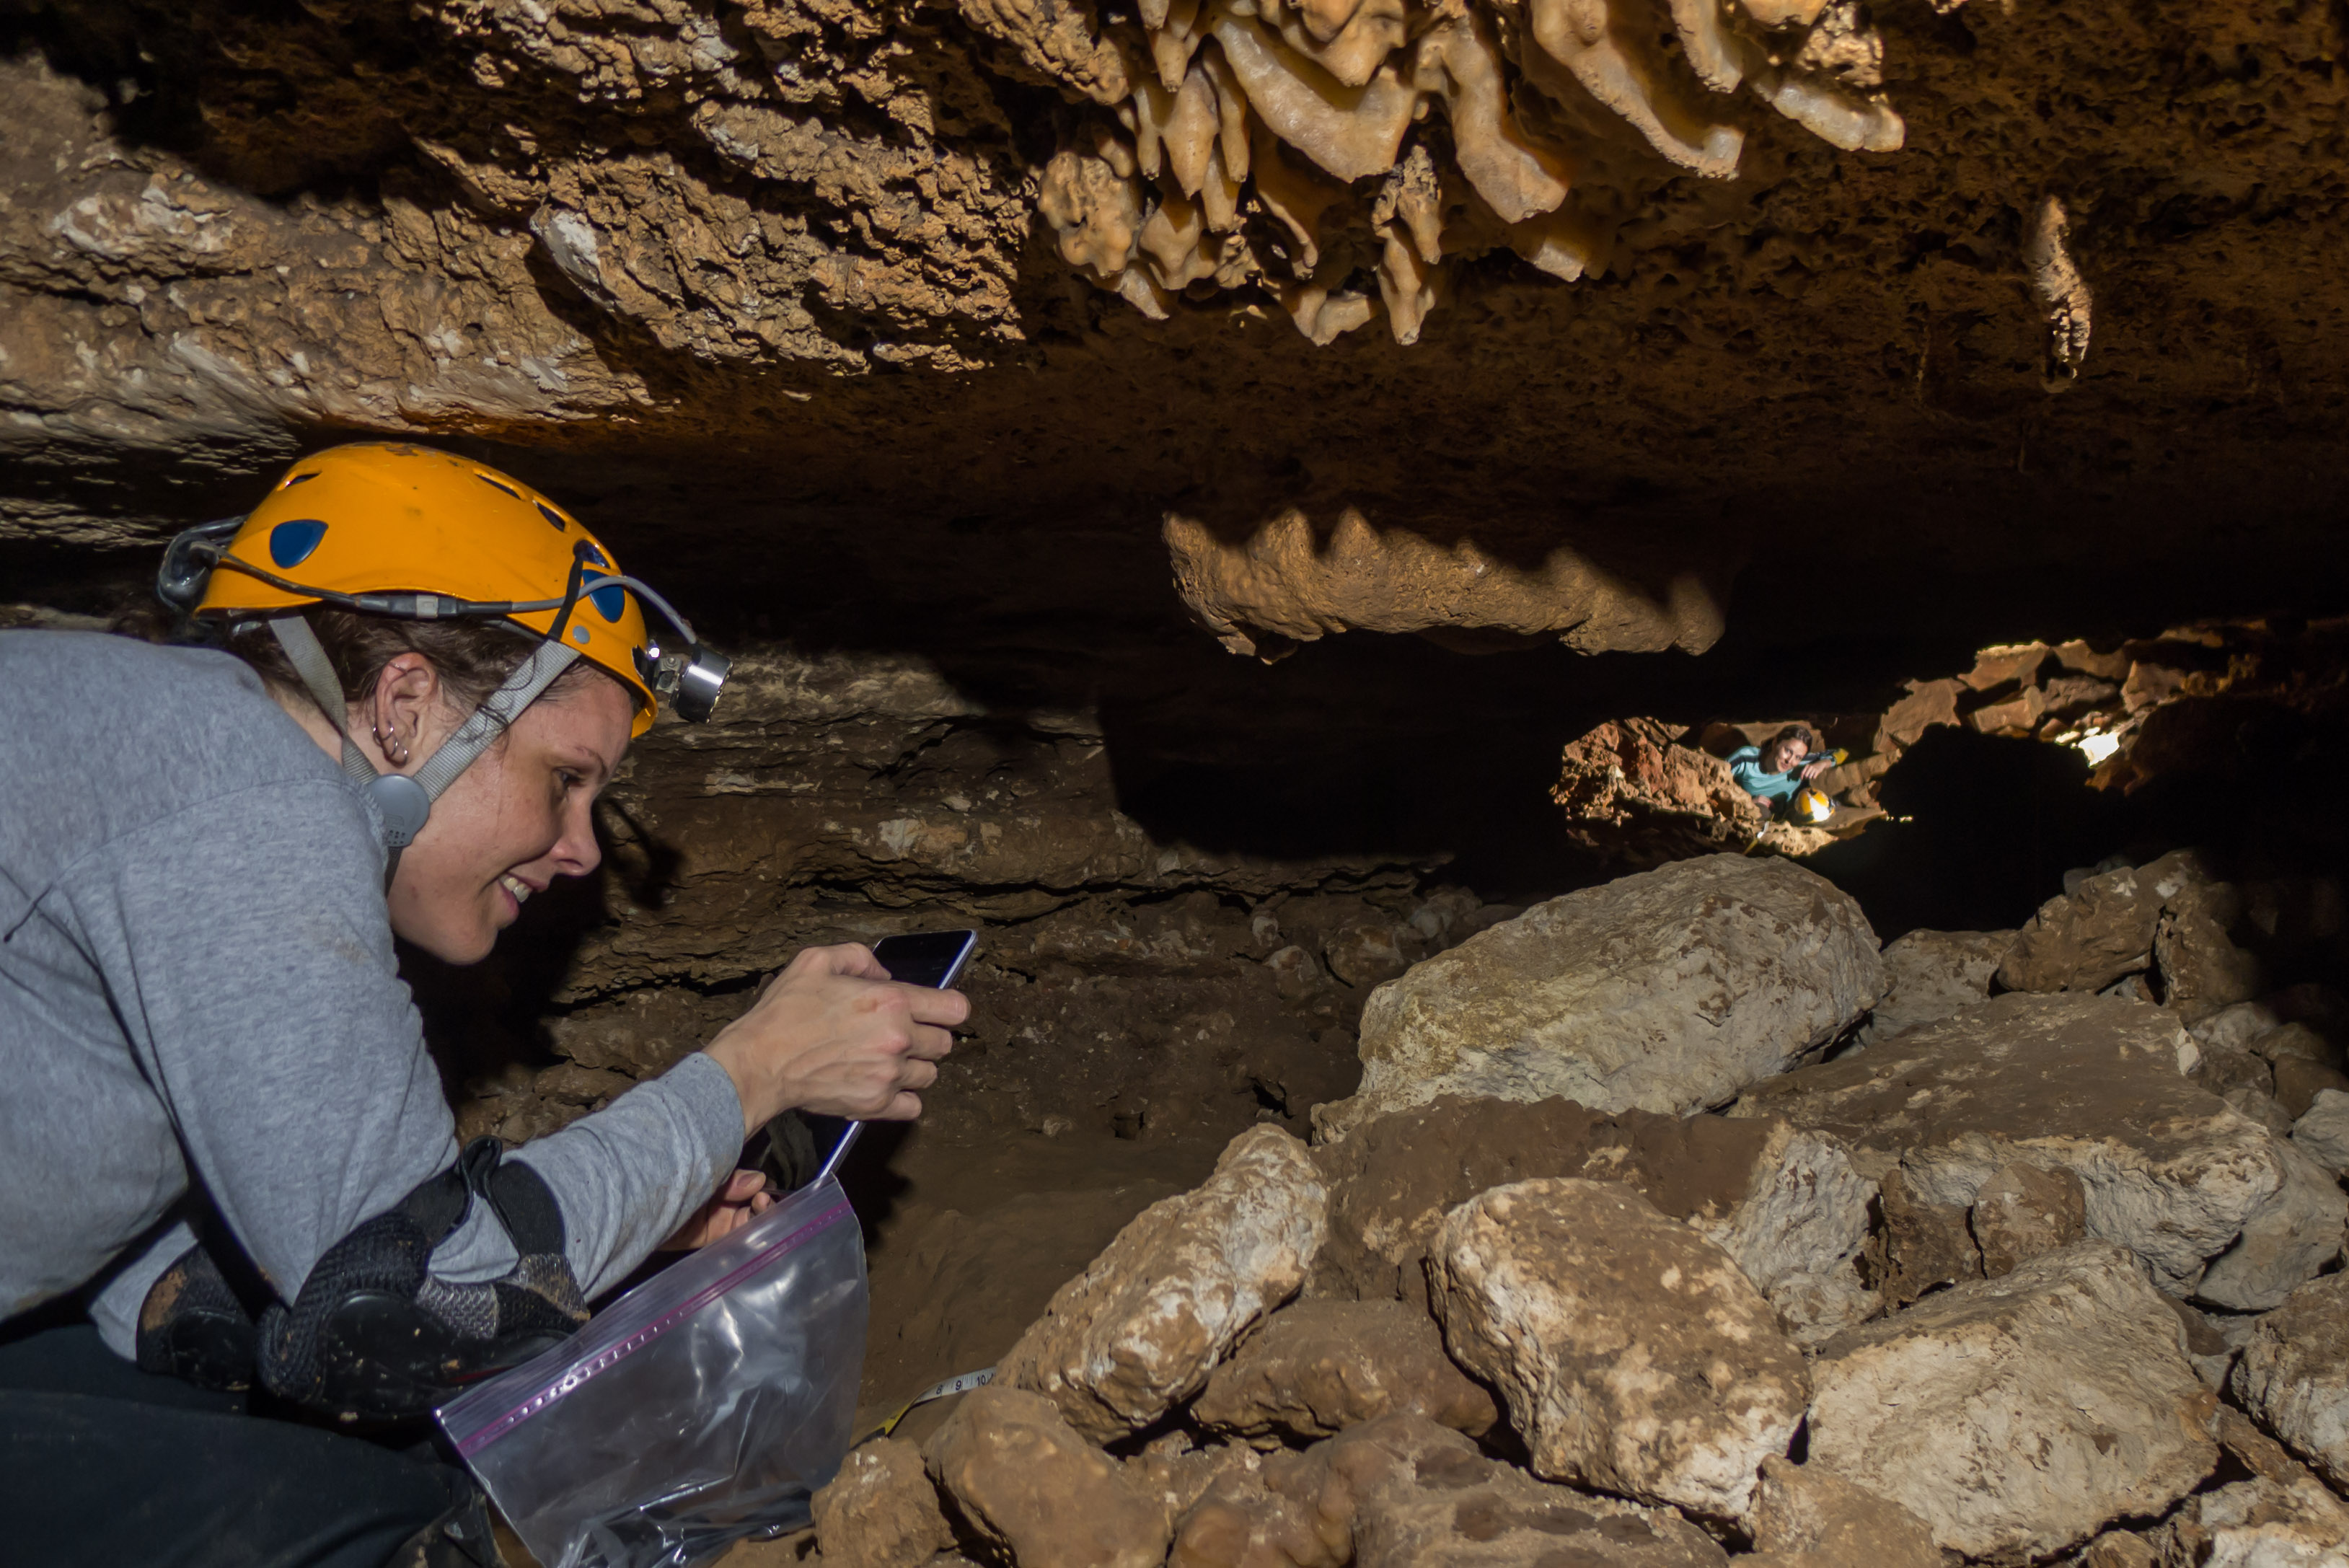
\includegraphics[width=\textwidth]{cavewifi2}
\caption{Testing WiFi Direct range in Whirlpool cave. \textit{Image courtesy of David Ochel.}}
\end{figure*}

\subsection{Outline of WiFi Direct Investigation}
\label{sec:Outline}
We propose an application using WiFi Direct enabled devices to automatically ferry data collected by sensors from within a cave back to the surface.
An automated data ferry application would be a far more convenient, effective, and safe mechanism for data retrieval versus current techniques.  
The WiFi Direct standard provides infrastructure mechanisms for discovery, addressing, and security. 
This infrastructure allows applications a simple and power effective means of setting up the network and transferring data. 

We will focus on two key questions in this paper regarding the potential of the WiFi Direct technology for this application.
\begin{enumerate}
\item Does WiFi Direct provide an effective range in a cave environment?
\item Can WiFi Direct, as provided by the Android platform, be used to form and disolve connections automatically to ferry data files from device to device.
\end{enumerate} 
WiFi Direct theoretically provides a range of up to 200m, which is greater than that of Bluetooth technology. 
We would like to determine the potential range of WiFi Direct specifically in a cave environment.
A cave environment is distincly different from a usual surface environment in that there are significantly more obstructions between devices. 

The still nascent implementation of the WiFi Direct standard poses some potential limitations for our use case.
Since the data will need to travel from device to device beyond the range of a single WiFi Direct group, 
each device will need to participate in one or two groups. 
The current implementation of WiFi Direct on Android devices does not allow a device to be simultaneously connected to two WiFi Direct groups.
Therefore, our prototype application will manage the disconnection from one group and connection to the next group automatically.

In addition, the current WiFi Protected Setup (WPS) implementation requires the human user of the device to approve any new connections.
Once a device has gained user permission once to a join a group, the Android platform "remembers" the credentials for the device and allows the device to automatically rejoin that group without user intervention.
Since we want our devices to be able to operate autonomously, we will show how to accommodate the approval issue by manually pre-configuring the devices for connections.
This allows the devices to bypass the step of a user key press when initiating a connection.
 
For the first phase of this project, we created a prototype application for Android devices. 
We used this application to test the ability to make WiFi Direct connections within Whirlpool Cave, a popular cave in south Austin with a variety of passage characteristics. 
The ultimate goal of this initial application and the cave excursion is to determine if the range and bandwidth of WiFi Direct is sufficient to support passing messages out of the cave.
The results of this initial testing showed that WiFi Direct had significant range in areas of the cave where direct line of sight was achievable between devices.
Just as a note, in typical surface environments, WiFi signals do not require direct line of sight as they can travel through common building materials.
However, the radio waves of WiFi signals cannot travel through substances like rock or concrete.
This fact could render this technology difficult to use is very narrow and winding caves.
We will discuss these experiments in Section~\ref{sec:WiFi Direct Range in a Cave}.

For the second phase of the project, we developed a second Android application to demonstrate how to pass a sample data file from device to device in a manner similar to how data would be ferried out of a cave.
Ultimately the second application successfully demonstrates that passing data from peer to peer in an automated fashion is achievable using WiFi Direct. 
In the development of this application, we built code to manage a device's participation in multiple WiFi Direct groups.
We also spent considerable effort managing timing, connection, and synchronization issues between the devices.
We explain these issues later in the paper, and we consider these issues to indicate areas of future work for middleware solutions
such as the Android platform.

\section{Related Work}
\label{sec:Related}
Cave explorers and researchers need in-cave communication systems in order to carry out complex group tasks such as expedition management, rescues, or photography projects.

Wired telephone technology is popular with expedition and rescue teams because they are simple and robust \cite{cavecomm}.
However, one major drawback of wire based systems is that the wire must be carefully laid along the cave passage. 
The wires themselves are heavy to carry and expensive.
Also, if the wire is broken somewhere along the line, then the entire system will not work.
Therefore, the drawbacks of wired telephone technology are the cost and weight of the wire and fragility of the system.

The APRS Cave-Link system is capable of sending text based messages via VHF/UHF walkie talkies or relay boxes placed along a cave passage.
In their experiments in a large cave, the average hop length was an average of 390' and 440' for VHF and UHF respectively.
The advantages of this system over wired systems are that the radio units and relay boxes are approximately hand-sized and are relatively lightweight.
The authors were using the system to essentially send text messages and did not address the general data capacity of the system \cite{cavelink}.

In Postojna Cave in Slovenia, a research team created a system for delay tolerant automatic data transfer from environmental monitoring systems deep in the cave.
Postojna Cave has a train to ferry tourists 2km into the cave.
Their system treats this train as a data mule by equipping it with a WiFi enabled computer which connects to monitoring stations inside the cave as the train passes by \cite{postojna2014}.
Overall, this is a very interesting approach. 
However, it requires a cave with regular traffic of some type to act as the data mule.

Moore, et al \cite{moore2012} considers using autonomous mobile radio nodes to connect a base station to a leader node via WiFi in tunnel exploration. 
Tunnel environments share some similarities with cave environments in that the passages usually consist of rough, concrete (rock-like) walls with straighter, longer passages of more consistent dimensions. 
Therefore, their experiments with WiFi signal attenuation in the tunnel environment give us useful data to use in predicting range possibilities in a cave environment.

\section{WiFi Direct and Android Support}

\subsection{WiFi Direct Overview}
\label{sec:WiFiD Overview}
Today, wireless connectivity is largely taken for granted. 
However, there are still a few circumstances that remind us that the Internet and general network connectivity are not guaranteed. 
Occasionally device connectivity to the broader Internet cannot be achieved due to physical, environmental, or technological constraints.
The WiFi Direct standard is one means of potentially filling that gap. 
In some use cases, broader connectivity to infrastructure is not required and there is value to simple device to device communication. 
This is WiFi Direct's niche, those circumstances where a broader infrastructure is either unavailable or unnecessary, and device to device communication is needed.

WiFi Direct is a standard developed by the WiFi Alliance which provides a mechanism for peer to peer communication in the absence of a dedicated wireless infrastructure. 
This standard has several benefits, first and foremost being that it does not require a dedicated wireless access point \cite{whywifid}, therefore users don't have worry about a DHCP server or other infrastructure pieces to enable their communication. 
In addition, this standard runs on typical wireless hardware found in all mobile devices, and is supported by most of the major mobile platforms such as Android 4.0, IOS 7, Blackberry, Windows 8, and even Xbox. 
Speed and range for WiFi Direct are those of typical WiFi devices and can operate at 250 Mbps and up to 200 meters depending on the environment. 
WiFi direct utilizes WPS and WPA-2 to ensure security of the communications over the peer to peer network. 
Since power management is especially important for mobile devices WiFi Direct includes power management mechanisms that can reduce power consumption for devices regardless of role.
All of these benefits make WiFi Direct an ideal selection as the technology for ferrying data from an underground cave.

The basic concepts of WiFi Direct are as follows. 
The WiFi Direct Group is a core component of WiFi Direct. 
The WiFi Direct group basically functions as an infrastructure basic service set (BSS). 
All components that can connect into a wireless medium in a network are referred to as stations. 
The BSS is a set of all stations that can communicate with each other. 
An infrastructure BSS includes both access points and stations in a wireless connection scenario \cite{wirelesslanwiki}.
All WiFi Direct devices must be capable of becoming the group owner. 
Within a group, a single device takes on this role.
 
The Group Owner is responsible for controlling which devices are allowed to join a group, when the group is started and terminated, BSS functionality, WPS Internal Registrar functionality, and communication between Clients in the Group. 
The Group owner decides if the group is temporary or persistent. 
A persistent group may be formed again without reinitiating WPS.
Group owners may optionally provide features such as simultaneous (concurrent) connection with an infrastructure network and sharing of that infrastructure connection. 

In addition to being able to execute the group owner role, WiFi Direct devices must also be capable of group ownership negotiation, discovery, and power management functions.
Devices adhering to the standard enter into a discovery phase where peers within range are found. 
Once a list of peers is retrieved, devices wishing to connect may either form a new  WiFi Direct group or connect to an existing group. 
As part of the group formation process, the devices wishing to connect establish which device will become the group owner.

A device obtains the role of group owner through one of three mechanisms: Standard, Autonomous, or Persistent. 
With Standard, devices negotiate to become the group owner.
With Persistent, a device identifies that a peer has been established as part of a past group. 
The group can be reformed, and the formation process can occur with a significantly reduced WPS phase because credentials for the devices have been stored.
With Autonomous, a device declares itself a group owner without involvement from any other peer devices. 
As part of providing the BSS functionality for the network, the group owner is responsible for providing DHCP addresses to devices on the network.
Data I/O can be handled via typical TCP/IP sockets, using the DHCP address provided by the group owner once the group is established \cite{wifiwhitepaper}.

WPS is used to obtain credentials and authenticate the WiFi Direct device as part of the connection process.  
This type of security requires user intervention in the form of the user either pushing a button or providing a PIN on the device.
The group owner generates and issues the security keys to other devices in the group to execute WPS. 
WPS, based on WPA-2 security, uses Advanced Encryption Standard (AES)-CCMP as cipher and a randomly generated Pre-Shared Key (PSK) for mutual authentication \cite{wifiwhitepaper}.
After WPS phase, devices disconnect and reconnect using their new authentication credentials.
When using persistent groups, credentials will be stored by the devices.
Therefore, the previous process of establishing authentication and manual user approval can be skipped, and the two devices can use their stored credentials to connect.

\subsection{Android APIs For WiFi Direct}
\label{sec:Android APIs For WiFi Direct}
We used the Android platform to evaluate WiFi Direct for the Swift use case.
Starting with Android 4.0 (API 14 and higher), Android provides three main areas within their API to support WiFi Direct:
\begin{enumerate}
\item The Wifi Manager 
\item Listeners 
\item Intents
\end{enumerate}
The WiFi Manager class provides methods to allow you to interact with the WiFi hardware on your device.
With the WiFi Manager you can do things like discover and connect to peers. 
Listeners allow you to be notified of the success or failure of WifiP2pManager method calls. 
Intents notify you of specific events detected by the WiFi P2P framework such as a dropped connection or a newly discovered peer. 
Actual data transfer between devices is handled by standard TCP/IP socket objects and I/O operations.
Android devices making use of the WiFi Direct functionality are required to request application permissions for: ACCESS\_WIFI\_STATE, CHANGE\_WIFI\_STATE, ACCESS\_NETWORK\_STATE, CHANGE\_NETWORK\_STATE, and INTERNET. \cite{androidoverview}

An application wishing to utilize WiFi Direct should implement several components to handle discovery and connectivity to peer devices.
The application must setup a Broadcast Receiver. 
A broadcast receiver allows you to receive intents broadcast by the Android system. 
In this case the application should respond to WiFi peer to peer intents.
The broadcast receiver must implement the necessary function calls to handle these intents in the Broadcast Receiver's "onReceive()" method.
The application will register the broadcast receiver and intent filter for the WiFi peer to peer events.
The application also should set up a peer to peer manager. 
The peer to peer manager known as "WifiP2pManager" class will be instantiated in the application, and it will be used to create a channel which will be passed to the broadcast receiver.

The peer to peer manager created for the application invokes the "discoverPeers()" method to discover peer devices.
Discovery is asynchronous, so an Intent is used to notify the application when discovered peers are available.
Once the application receives notification of available peers, the broadcast receiver component can query the peer to peer manager for the list of available peers by calling the "requestPeers()" function.
This function call is also asynchronous, and the function "onPeersAvailable()" which is implemented in the PeerListListener is executed when the "requestPeers()" function succeeds. 
The result is a list of WifiP2pDevice devices with which a WiFi Direct connection can be made. \cite{androidp2p}

The application invokes the "connect()" function provided by the WiFi peer to peer manager to establish a connection to a selected device.
The "connect()" function takes WifiP2pConfig object as a parameter which can include details from the WifiP2pDevice such as the device's address.
The "connect()" function is another asynchronous call. 
An application is informed of a successful connection, or WiFi Direct group formation, when the "onConnectionInfoAvailable()" functions is called.
At this point, the WiFi Direct group has been formed, or reformed, and the device is ready to transfer data using socket methods.

\section{Experiments}

\subsection{Typical Sensor, Data Logger Usage and Data File}
\label{sec:TypicalUsage}
Wong, et al carried out their experiments with a Telaire 7001 CO2 Sensor \cite{telaire} \cite{wong2010}. 
This is a hand held CO$_2$ and temperature sensor.
This sensor can perform environmental readings, but it cannot save data.
To save data from the sensor, you must attach it to a compatible logger.
HOBO offers a variety of loggers.
Some loggers have a USB output; others have WiFi, Cellular, or Ethernet communications.
In a cave, none of these connections is usually possible, so I suspect most research teams opt for the less expensive systems without external communications.
An example inexpensive logger is the HOBO U12 4-Channel External Data Logger equipped with 64K bytes of memory which is enough for 43,000 12-bit measurements \cite{logger}. 
%Some data loggers do have larger memory capacities such as 4mb (todo: cite other logger).
%Just commenting this until it is here, in case we forget the todo won't show in the final paper.

Based on the Wong paper and informal interviews with cave researchers, we learned that a cave research project will typically use one or a few similar sensors and attached data loggers.
Researchers will attempt to gather their data balancing retrieval frequency so data loggers neither overfill nor are the cavers burdened by the overhead of excessive caving trips.
Of course, we hope to reduce the caver's burden with WiFi Direct technology.
However, for the sake of our research, we needed to understand the typical experiment setup.

Zara Environmental gave us an example data file gathered from a logger and sensor setup that was measuring various environmental features like temperature, wind speed, pressure and so on.
This file has about six weeks worth of data and is 305K in size \cite{datafile}.
Therefore, we considered this a good example of the kind of data our application would be required to transmit in real life.
We used this data file in all of our experiments and have included a copy of it in both applications.

\subsection{Methodology for Measuring Range and Connectivity}
\label{sec:Methodology}
WiFi Direct operates on the same 2.4Ghz band as most 802.11 based WiFi deployments \cite{wifiwhitepaper}.
Typical indoor deployments of 802.11[bg] have a range of 35m, and outdoor deployments can have a range up to 100m.
802.11n deployments can have up to twice that range \cite{wikiwifi}.

We found various sources on the internet claiming that the range of WiFi Direct was anywhere from 10m to 200m. 
Of course, the achievable range of the WiFi Direct signal can and should vary depending on the topology of the environment, how many other devices are trying to use the same WiFi band, and of course any obstructions between the devices trying to communicate.

We designed experiments to evaluate the range of WiFi Direct between our devices in the most ideal deployment environment possible and in an example cave environment.
For each connectivity and transfer experiment, we followed the same procedure. 
We started with the devices not connected, but with the WiFi Direct group already established.
First, the user of one device would initiate a connection.
Once connection succeeded, we would perform three file transfer attempts using the response of the app to verify the success of each attempt.
Last, we disconnected the device, and moved to a new position for the next experiment.

\begin{figure}
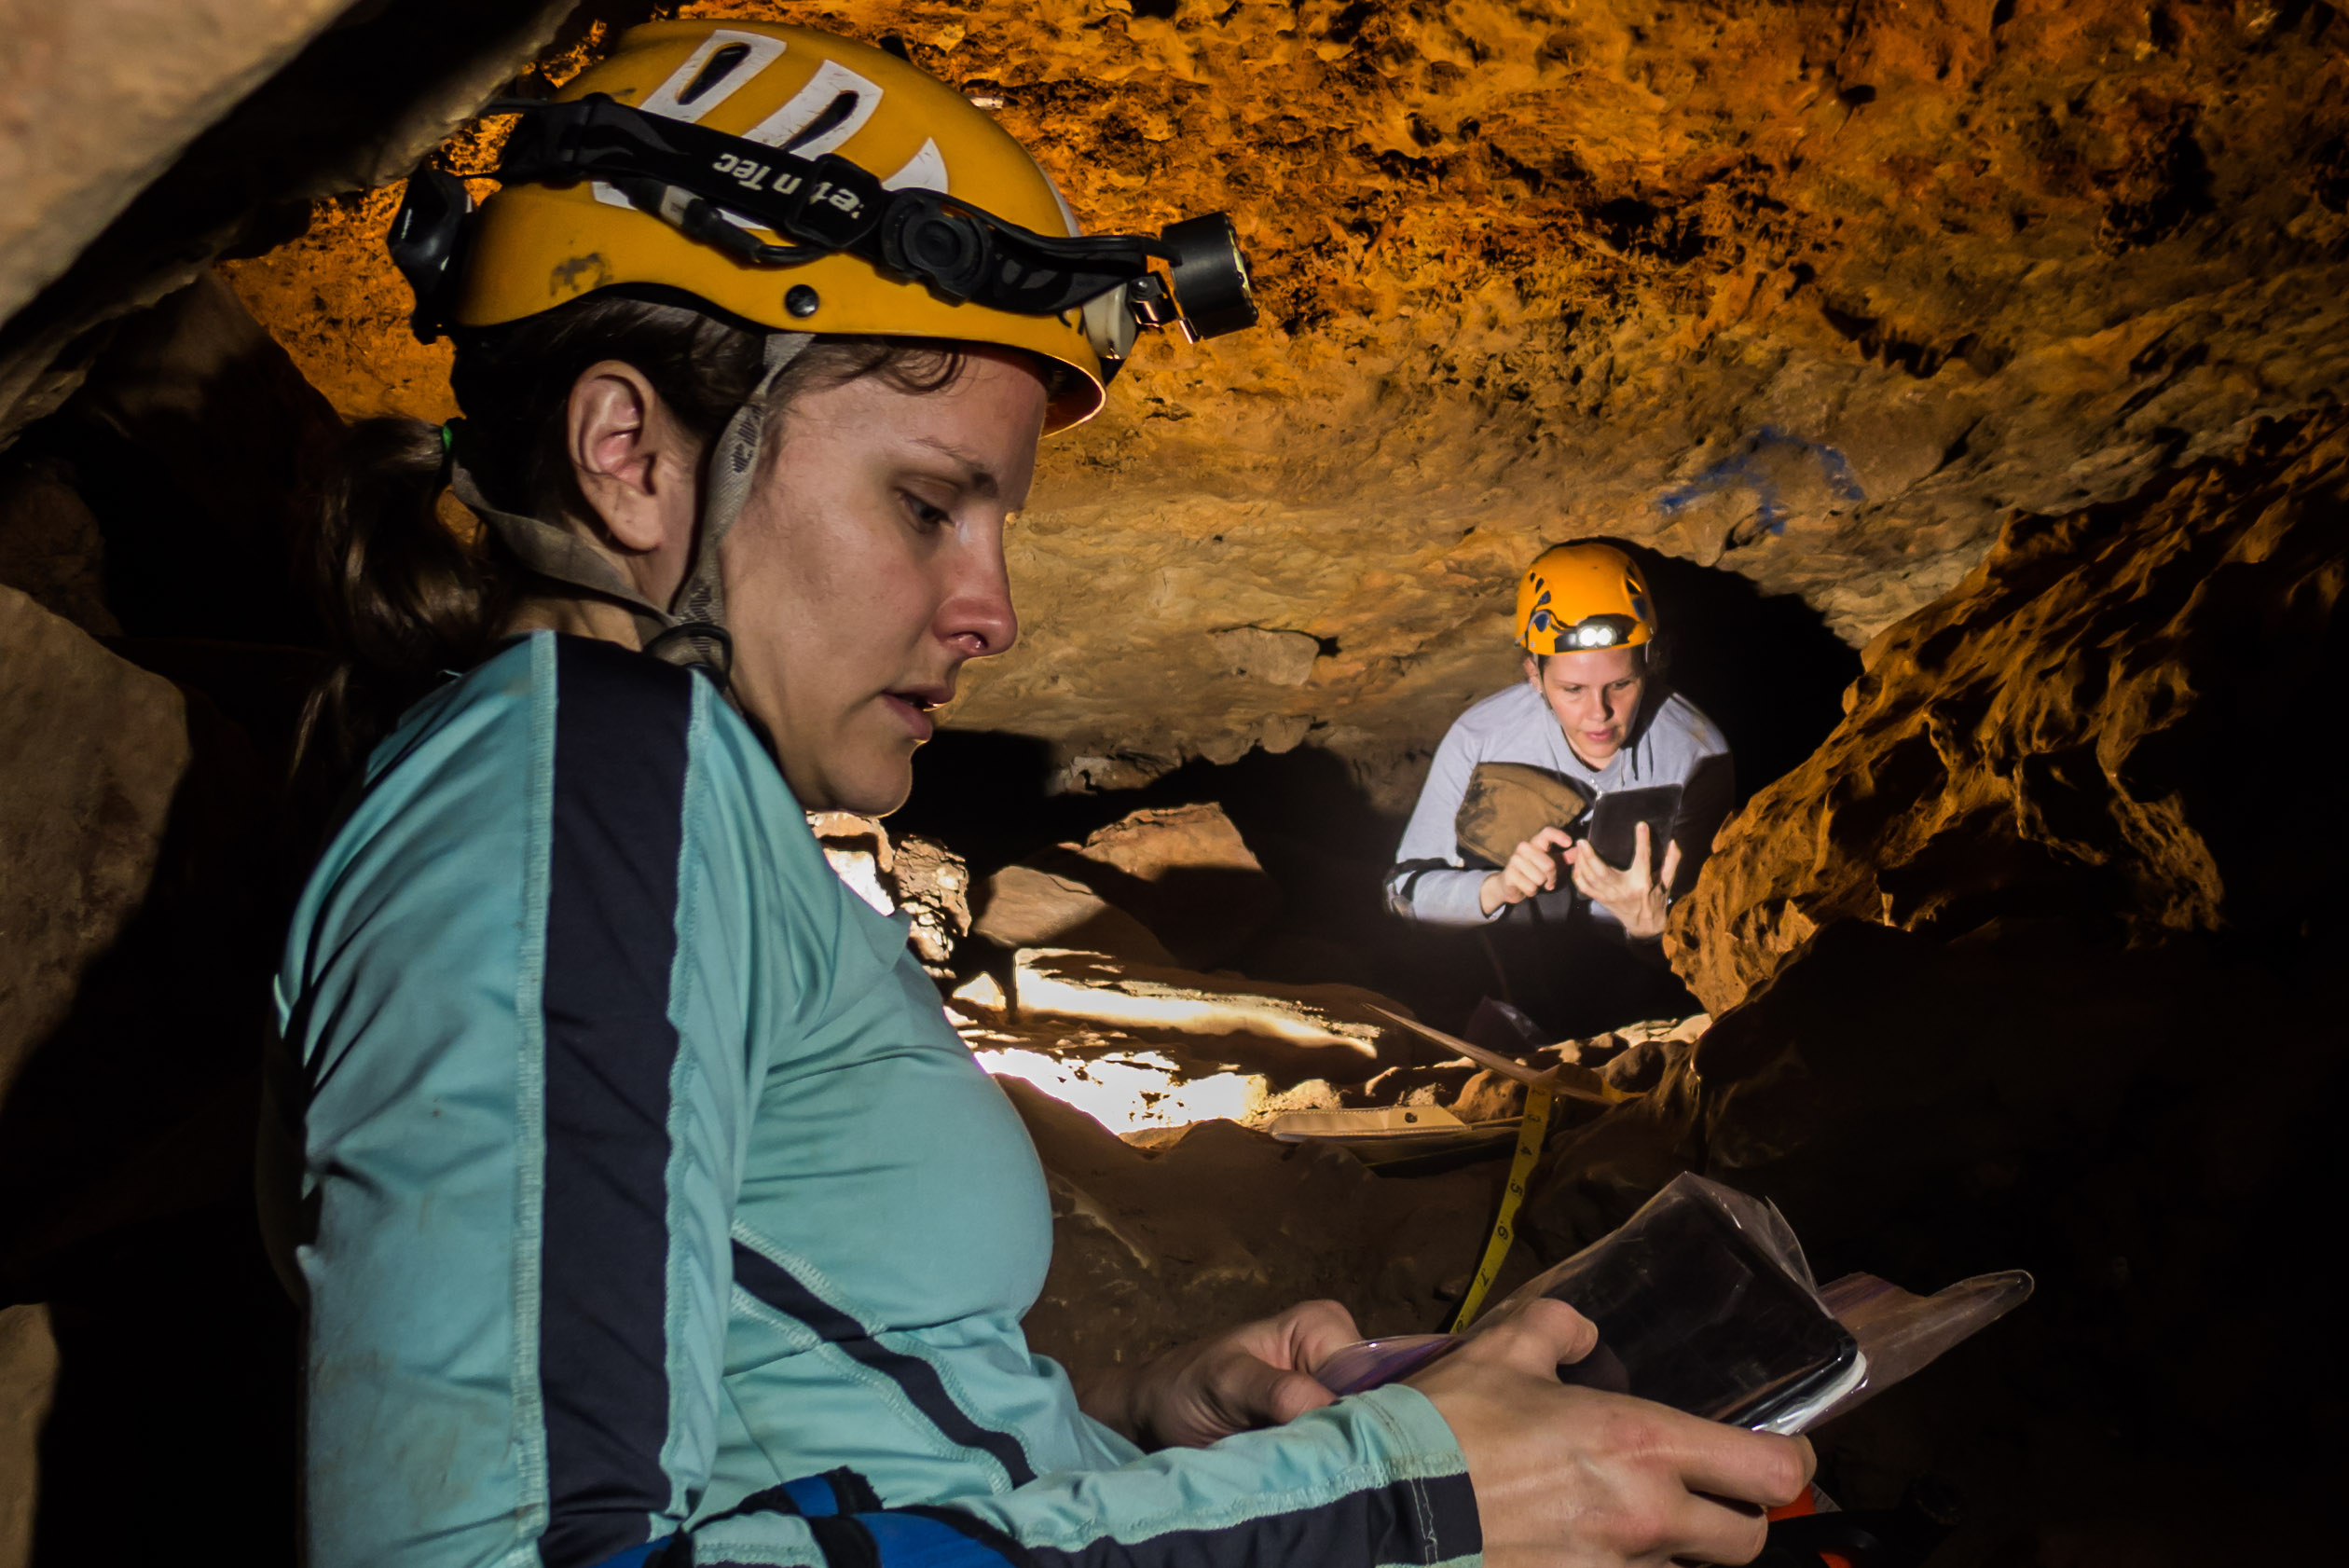
\includegraphics[width=\columnwidth]{cavewifi}
\caption{Testing WiFi Direct range in Whirlpool cave. \textit{Image courtesy of David Ochel.}}
\end{figure}


\subsection{Range Experiment Software}
\label{sec:Range Experiment Software}
Using the WiFi Direct example provided by the Android SDK, 
we developed an Android application to perform the range experiments in a cave.
Using this application we tested distances that could be achieved by WiFi Direct on a mobile device.
This example application taught us how to create the necessary WiFi Direct components and how the significant asynchronous function calls operate together.
To perform the range experiments, we modified the example to open a connection to another device, load a data file from the device, and send the data file. 
The example application and our derived application followed the architecture described in Section~\ref{sec:Android APIs For WiFi Direct} for creating peer to peer connections. 
Either application presents a simple GUI interface allowing the user to kick off discovery of peer devices. 
Upon completion of discovery the GUI displays a list of available peers.
The user can then select a device from the list of available devices which brings up a menu to connect to that device.

Once the WiFi Direct connection is established, the user may either disconnect or, optionally, select a button to transfer the data file.
The device selected as the "group owner" during the negotiation process is the receiver of the file, and the other device is the sender of the file.
There is no technical reason for this distinction; it is just how the example application was configured.
The device which is designated to be the receiver has slightly different functionality.
It has the option of terminating the connection and, in our derived application, a button to reset the socket in order to receive the next data file.

We added a log file to our application to capture the time required to send or receive a file just for further information.
The application timestamps the start and end of the data transfer, calculates duration, and logs this information to a log file.
In addition, the GUI of our application allows the user to enter a note to be included in the log file to help identify the test being performed at the time.

We developed this application in order to test the ability to establish a connection throughout the cave and to verify the successful transfer of the full data.

\subsection{Data Ferry Software}
\label{sec:Data Ferry Software}
In the second phase of the project we designed and built an Android application called SwiftDataHop to automatically transfer a data file sequentially from device to device. 
This project leveraged some of the WiFi Direct data transfer code from the range software and implemented a state machine to allow the application to execute in "Operate Mode" where data hops automatically from device to device. 
To utilize Operate Mode, the user must configure each device to identify device roles and execute WPS to store credentials.
During this project the application did not interface to an actual data logger.
Instead, a datalogger was simulated with a pre-populated data file.
The application was notified to intiatiate the transfer of the pre-populated data file via a button click on the user interface.

SwiftDataHop has two modes of execution: Manual Mode and Operate Mode.
Manual Mode has the same connect and transfer capability as described in the range experiment software.
In addition, a user runs in Manual Mode to initiate WPS between devices so that user intervention is not required during Operate Mode to accepta a connection.
In this mode, devices are identified as upstream and/or downstream and this configuration can be viewed or reset if necessary.
A downstream device is a device from which a file is received, and an upstream device is a device to which a file is sent.

A device can have one of three roles: 
\begin{enumerate}
\item Data file initiator
\item Sender-receiver
\item Endpoint
\end{enumerate}
A device's role is determined by whether a single upstream, a single downstream, or both an upstream and downstream device are set.
A device with no downstream device set is a data file initiator and will have the capability to initiate the file transfer of the data file in Operate Mode.
A device with both an upstream and downstream device is a sender-receiver and will wait for a connection from a downstream device, receive a file, disconnect from the downstream device, connect to an upstream device, and then send the received file.
A device with no upstream device is an endpoint, and will display the file received and location to which it is copied on the file system.

Operate Mode is the automated mode of the application.
A device cannot enter Operate Mode without at least one upstream or downstream device set.
The application may be in one of four states: OFF, IDLE\_WAIT, SEND\_FILE, and RECEIVE\_FILE.
The OFF state means that the application is in Manual Mode.
Figure 3 shows the states, key state activities, and the transition conditions for each state.

When Operate Mode is entered, the device initially goes into the IDLE\_WAIT state.
There are three possible ways to transition out of the IDLE\_WAIT state:
\begin{enumerate}
  \item When someone clicks the button to disable Operate Mode, the application transitions back to the OFF state.
  \item When someone clicks the button to "Send File", which is enabled on a device with only an upstream device set, the application transitions to the SEND\_FILE state.
  \item When a WiFi Direct Group is initiated from a downstream device, the upstream device transitions to the RECEIVE\_FILE state.
\end{enumerate}
\begin{figure}
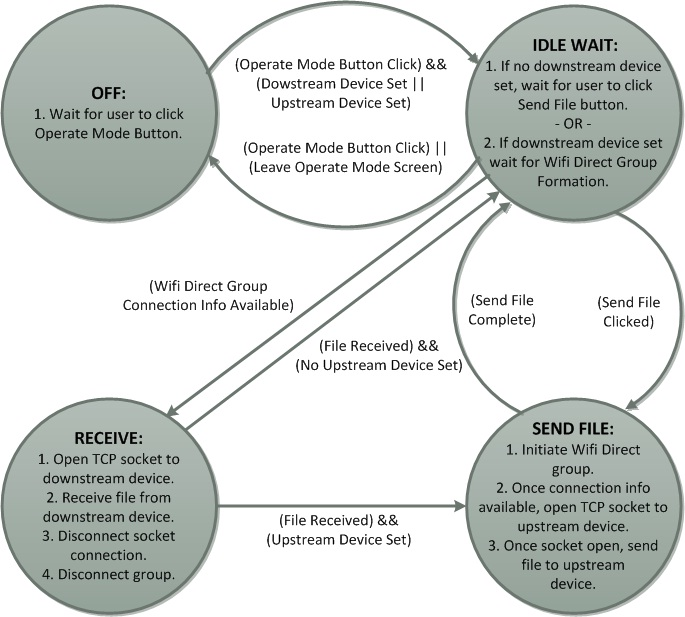
\includegraphics[width=\columnwidth]{statemachine}
\caption{Operate Mode State Machine.}
\end{figure}
If a device is in the SEND\_FILE state, after operations are performed to send the data file upstream, the device will return to the IDLE\_WAIT state.

If a device is in the RECEIVE\_FILE state, it will perform operations to receive a file, and then if an upstream device has been configured it will transition into the SEND\_FILE state.
If an upstream device has not been configured, it will transition back to the IDLE\_WAIT state as that indicates it is the final device in the transfer.

The operations to send and receive a file can be broken down into the operations required to execute WiFi Direct group formation, create a socket connection, and perform a file transfer. 
Once the send file button is clicked and a device goes into the SEND\_FILE state, it initiates a WiFi Direct "Connect" which is handled by Android APIs.
Both devices are notified of the successful group formation by the "onConnectionInfoAvailable" callback.

A small, arbitrary delay is injected here to give the upstream device an opportunity to be available for a socket connection.
After this delay, the downstream device creates a TCP socket connection to the upstream device using the connection info returned from "onConnectionInfoAvailable".
Once a successful connection is established, the file data is written to the socket, the socket connection is closed, and the WiFi Direct group is disconnected.
The sending device returns to the IDLE\_WAIT state.

Upon WiFi Direct Group Formation, the upstream device enters the RECEIVE\_FILE state and immediately opens a socket for the downstream device to connect to.
Once a connection is received, the device reads the data file from the socket, closes the socket, and disconnects the WiFi Direct group.
The receiving device then will transition to the IDLE\_WAIT state if it is an endpoint, or it will transition to the SEND\_FILE state in order to perform send operations if it has an upstream device.

%This seems out of place here. I think this probably better suited to the results section. 
%It is actually the timing and synchronization of the group formation, %subsequent socket connection, and file transfer that was the most tricky to %implement in the application.

\section{Results}

\begin{figure*}[t]
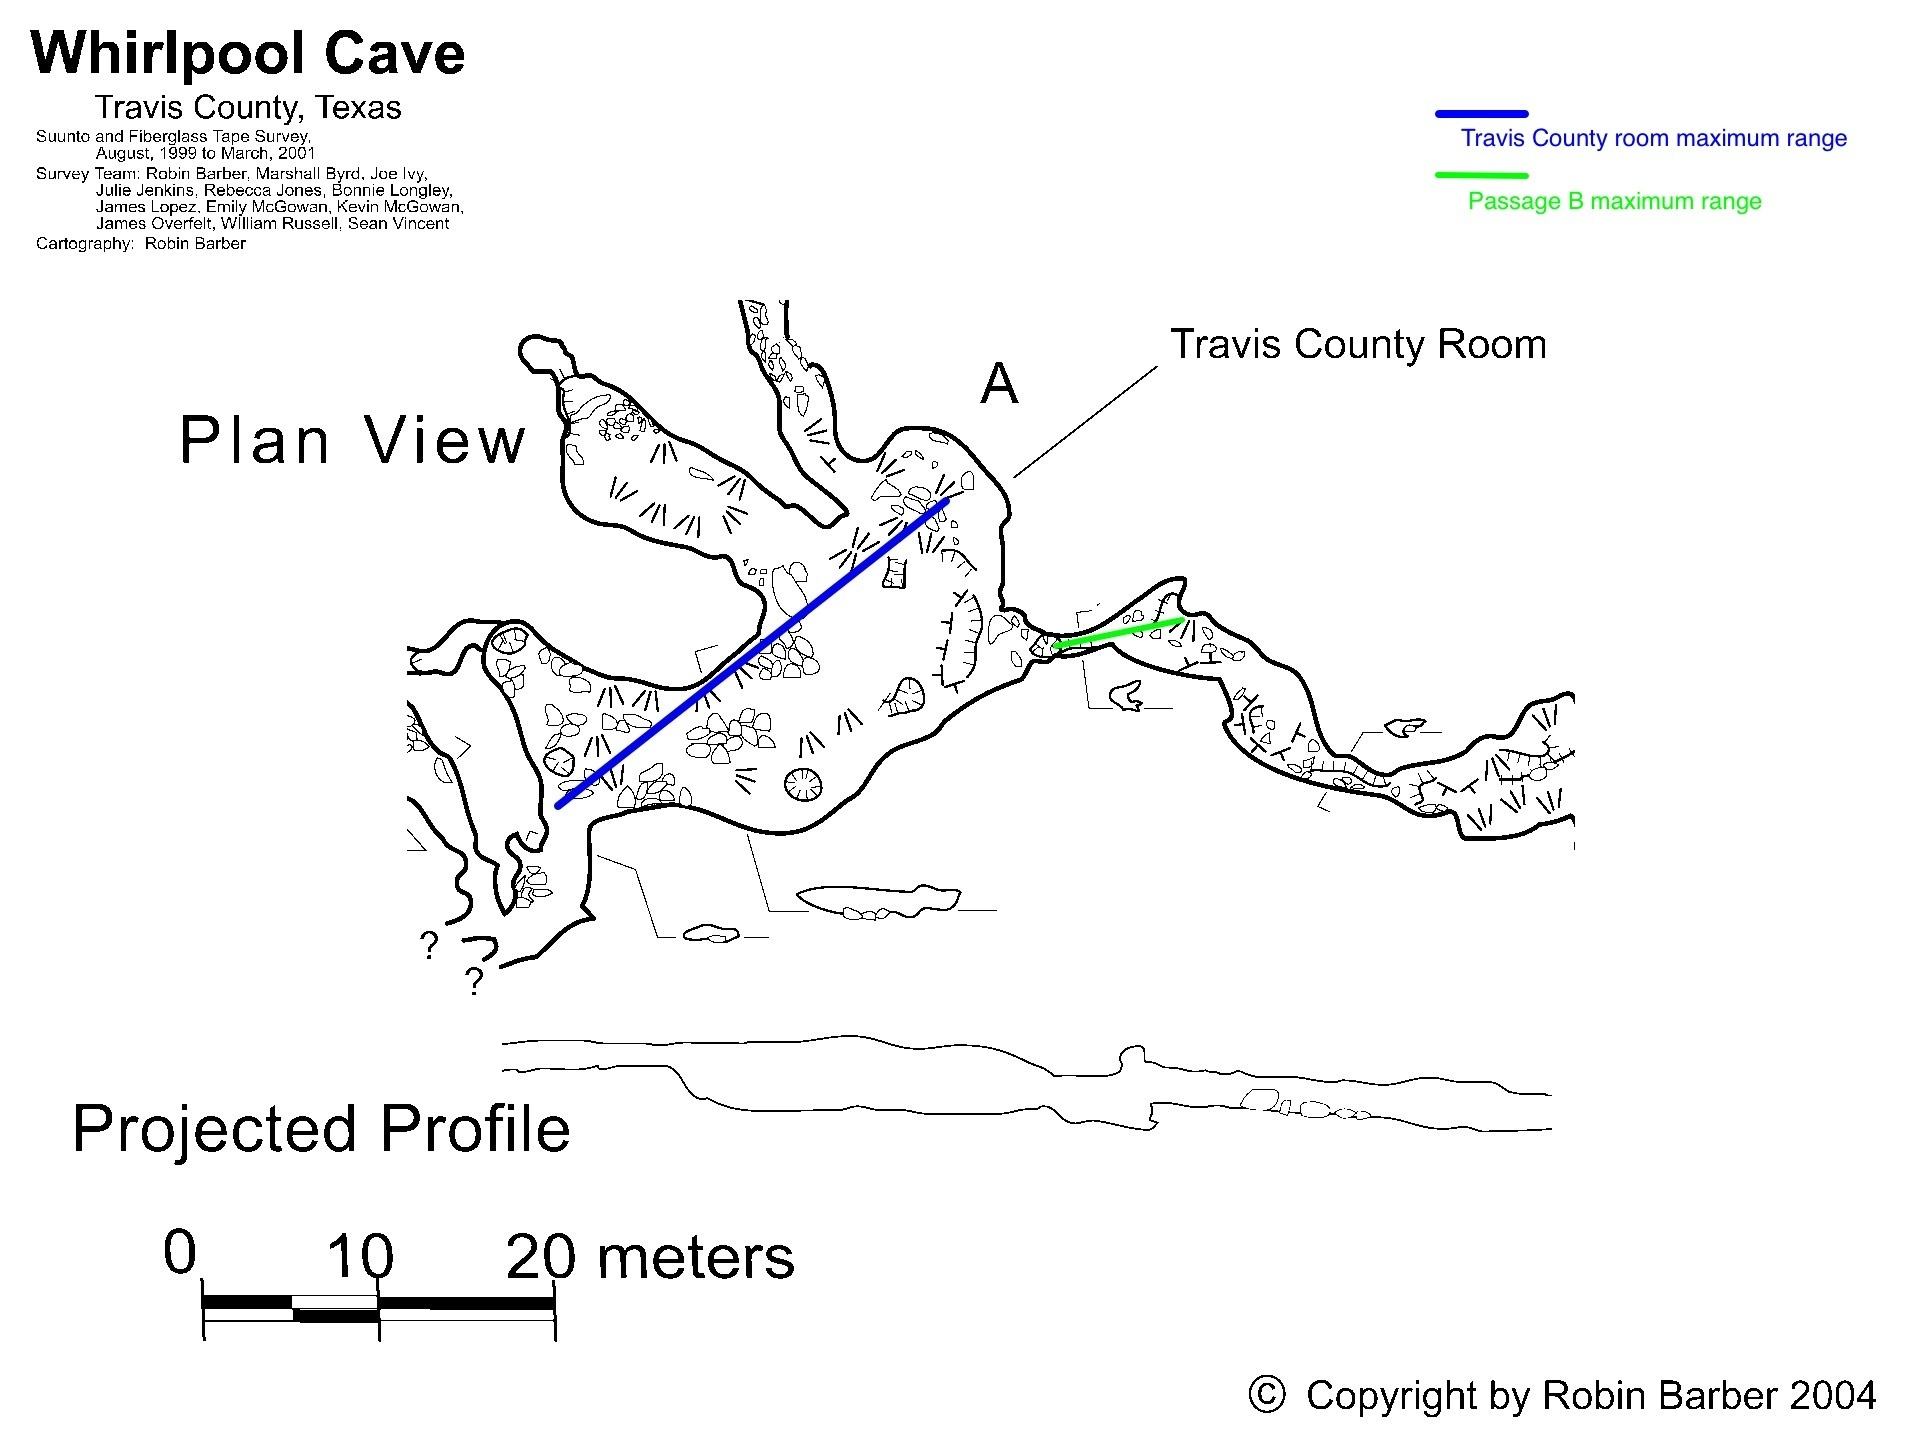
\includegraphics[width=\textwidth]{our_whirlpool_experiments}
\caption{Our achieved range in Whirlpool Cave. \textit{Excerpts from Whirlpool Cave map \cite{wp_map}.}}
\label{fig:whirlpool_map}
\end{figure*}

\subsection{WiFi Direct Range in Open Field}
\label{sec:WiFi Direct Range in Open Field}
We found a relatively open field in north Austin to carry out some range experiments with our Nexus 7 devices.
An open field, with no line of site obstructions and no other WiFi devices around, should be the most ideal setting for WiFi Direct ranges.
We started our tests at 100' apart and increased the distance by 50' to 100' at a time.
Our devices easily connected and transfered a sample data file at distances up to 300' (91meters). 
We were able to connect and send the sample file at 350', 400', 500', and 600' (183m) with moderate success. 
At times, the connection would take longer than usual.
Also, the initial file transfer took multiple attempts.
Once the initial file was received, then subsequent transfers went much better.
However, at 650' (198m) the devices had a lot of trouble connecting, so we stopped measurements at that point.
This is very close to the claimed range of 200' meters.

\subsection{WiFi Direct Range in a Cave}
\label{sec:WiFi Direct Range in a Cave}
We gained access to Whirlpool Cave in south Austin with the permission of the managing entity, TCMA (http://www.tcmacaves.org/) and experimented with the range and connectivity of our Nexus 7 devices on March 16, 2014.
Whirlpool Cave is a relatively typical cave for central Texas.
It has over 400m of total passage \cite{whirlpool}. 
Most of the passages are traveled by crawling.
However, an adult can stand in some of the larger rooms.

We began our range experiments in the largest room known as Travis County room which has the longest possible horizontal line of sight available in the cave.
In this room, our devices were able to easily connect and transmit test files at distances of 55', 80' and 97'. 
After 97' we were no longer able to achieve line of sight.
This distance represents nearly the maximum length of the room. 
Behind our respective survey stations, the ceiling and floor of the room quickly meet.

Next, we wanted to see how connectivity would fare in a smaller passage. 
We moved out of the Travis County room into the southerly passage known as 'B' on the map.
The height of this passage varied between 36" at the first position to 2.5' height at 28' feet distance.
We also measured a minimum height of 19" at one point in the passage between survey stations.
This passage is a few meters wide per the map, so we did not specifically measure that dimension as height was the limiting factor.
Our Nexus devices successfully connected at 8' and 28' feet apart.
After 28' apart, the passage starts to turn making line of sight was impossible to maintain, so our devices could not connect.
Furthermore, since this passage was so narrow and filled with rubble, we had to take great care to maintain a line of sight between the devices.

Please see Figure ~\ref{fig:whirlpool_map} for an illustration of the cave and where we performed our range experiments.

Since the cave offers neiher larger rooms nor longer passages, we had to cease our experiments in Whirlpool cave at that point.
However, we suspect that in a larger cave or with straighter passages longer range should be possible.
Moore, et al carried out WiFi range experiments in straight mine tunnels where they claim that signal loss attenuates there less quickly than in free space.
We refer you to that work for details.
We would like to state here that their work found that WiFi signals attenuated less quickly in a tunnel of 8' rough diameters versus a tunnel of 15' rough diameter, so we are optimistic about the range possibilities in longer cave passages. \cite{moore2012}.


\subsection{Data Ferry Experiment Results}
\label{sec:Data Ferry Experiment Results}
Section~\ref{sec:Data Ferry Software} covered the design of the WiFi Direct data ferry application called SwiftDataHop. 

The data ferry software prototype demonstrated that WiFi Direct could be used to pass data from device to device in an automated fashion. 
During the course of this project, our four Nexus 7 tablets running Android 4.4.2 successfully and automatically executed the transfer of a data file.
The project was limited to four devices simply by the number of available tablets.
Additional devices could be added to achieve further distances or deal with a larger number of topology challenges in the cave that could prevent line of sight connectivity. 
While the SwiftDataHop application executed the automated transfer across the devices, there are still several issues that need to be resolved before the application can be put to practical use.
Timing was a key challenge in implementing Operate Mode, or the automated mode of this application.
SwiftDataHop was tuned for our experiment with delays to allow for connection time, disconnect time, and file transfer completion.
For example, once the first phase of creating the WiFi Direct group was completed, the sending device would receive notification that the group was established.  
If the sending device opened its socket to the upstream device before the upstream device had time to open a socket and wait for connections, connectivity might fail.
Since the goal of the initial prototype was just to prove the feasibility of WiFi Direct technology in this type of application, there are likely better solutions such as implementing an acknowledgement mechanism or retries as opposed to injecting arbitrary delays into the process. 
In addition, the Android WiFi Direct APIs showed inconsistent behavior.
These APIs are very sensitive to other operations being performed on the device and offer little in terms of visibility and debug into the lower level system functions taking place on the device.
During the experiments for this project, the application could only execute a single automated transfer and then user intervention would be required to reset the device either by manually disconnecting from all devices or by disabling and re-enabling wireless services on the mobile device.
If we had additional time to dig into the source for the Android APIs, it is highly likely that the root cause of this issue could be found and overcome.
Behavior of the APIs became more predictable when all other wireless activity was disabled on the tablets.
This would be a reasonable constraint in the cave environment as no other wireless infrastructure would be available.
In summary, this application was an effective prototype to prove that WiFi Direct could be used to leverage peer to peer connectivity in the absence of infrastructure to act as a ferry for data from in-cave loggers.

\section{Conclusions and Future Work}

\subsection{Application in Cave Systems}
\label{sec:Application in Cave Systems}
\begin{figure}

\includegraphics[width=\columnwidth]{krubera_pit_dark}
\caption{Vertical passage in Krubera-Varonya \textit{Image found in article \cite{krub_blaze}}}
\end{figure}
We performed our WiFi Direct experiments in a cave easily accessible to us and fairly typical of caves in this part of central Texas.
%This sentence seems redundant?
Cave systems around the world present with a wide variety of morphologies, and a given cave system will usually contain a wide variety of morphologies within it.
Morphology examples include passages that are passable only to water and insects and, in contrast, passages that are the size of large buildings and navigable by commercial aircraft.
Passages are horizontal, vertical, or any angle between the two.
Some passages can be adequately described as enclosed, underground "rooms" or "pits" where the top is open to the sky.

We would like to theorize further about how our research might generalize to other caves and where this technology will have the greatest value.
WiFi Direct has several advantages including bandwidth, range, weight, and ease of deployment as we covered in Related Work, Section~\ref{sec:Related}.
It is important to note, that WiFi Direct signals only work in caves when a direct line of sight is available, and the devices require a consistent source of energy.
Therefore, we propose a few example scenarios where WiFi Direct could be particularly useful as part of an in-cave communication system.

The cave Krubera-Varonya in West Caucasus in Abkhazia, Georgia is presently the world's deepest cave system with a depth of nearly 2200m and with 13.4km of passage. 
Speleologists, cavers and cave divers have been exploring and mapping this cave since at least 1982.
Expeditions in this cave are complex operations where an example cave exploration trip will span multiple weeks with at least 19 people including cavers and cave divers.
On these expeditions, cavers will survey and map the cave; specially trained cave divers will proceed through and map underwater passages, place data loggers to measure water levels, and more.
The cavers will need to be underground for weeks at a time and stay in one or more of a handful of underground camps \cite{krub_it}.
A communication system to coordinate re-supply, logistics, and, in the worst case, coordinate a rescue operation is almost a requirement for an expedition of this magnitude.
While it is difficult to determine potential length of line of sight by looking at published photos and maps, 
it certainly seems quite possible that this cave has many passages that would be great candidates for using WiFi Direct.
Published photos and maps show that the cave has some very long (100m) vertical drops in large, fairly straight passages and some similarly large and long horizontal passages \cite{krub_it}.
Cavers train in specialized single rope techniques to ascend and descend such vertical passages.
Even given extensive training and experience, it takes quite a long time (multiple hours) for a team of cavers to ascend or descend long vertical drops particularly since those cavers are usually carrying very heavy gear and supplies.
Therefore, there is a great opportunity to ease the physical exertion and time burden if messages can be communicated at WiFi speed and bandwidth through such a passage.
Between WiFi direct points, communication could even potentially be as high fidelity as voice and video such as between the top and bottom of a particular pit.
Since this cave has several sections of very tight passage and underwater passages,
a realistic system enabling communication throughout the cave such as from camp to camp to surface would most likely need to be hybrid:
consisting of WiFi direct relays wherever practical to achieve distance with ease of installation, using single wire systems in winding passages, using underwater radio signals through sump passages (only passable by trained cave divers), and so on.
In such a hybrid system, our prototype application which can automatically transfer messages from device to device would be particularly helpful.

We can envision a purely WiFi direct cave system being used to enable communication in certain cases such as from a pit bottom to the surface.
WiFi Direct could also play a key role in a hybrid scenarios enabling communication through other extensive cave systems that are similar to Krubera-Varonya in size and complexity. 

\subsection{Future Work}
\label{sec:Future Work}
There are numerous areas that could be considered for future work that were out of scope for this project due to the time available.

During this project we did not focus on measuring or reducing power consumption.
Rather, we were focused on a showing that the WiFi Direct technology has the capability to automatically ferry data within a cave.
One reported advantage of the WiFi Direct standard over other ad hoc wireless connection standards is that it provides for better power efficiency during discovery and connect \cite{wifiwhitepaper}.
Therefore, the WiFi Direct technology is a good starting point for building a low power data ferrying solution.
Power conservation is very important in a cave environment as access to a power source is unlikely unless the cave is a tourist cave already outfitted with a lighting system.
We propose that future work in this area can reduce power requirements beyond what is provided inherently with WiFi Direct.
For instance, the data transfer can be done with smaller, lower power devices.
One way to reduce power consumption is to minimize the human interface component.
Specifically, large screens consume a lot of power, so realistic implementations could use a smaller screen or no screen.

Another area of future research will be to better coordinate the timing of data exchange in the interests of reducing power.
For example, data transfer does not usually need to be continuous or too frequent in our target use case.
The upstream devices in our implementation do not have any way to know when a downstream device might make a connection, so all devices remain active at all times.
In a realistic deployment, data transfer could take place on a relatively infrequent, such as daily or weekly, basis.
Therefore, a mechanism to incorporate preprogrammed periods for the devices to be inactive
and a time schedule for all devices to awake to do a scheduled data transfer would reduce power consumption.

As noted in Section~\ref{sec:Data Ferry Experiment Results}, it was difficult to get the timing of operations correct in the application due to the highly asynchronous nature of the required tasks.
In the prototype, we injected preconfigured delays based on our experiments to allow time for devices to complete known longer running tasks.
In the future a design including handshake, acknowledge, and retry could allow us to determine for certain that a device is in the desired state and ready before operations are executed as opposed to injecting arbitrary delays.

We did not connect to actual data loggers in our experiments although we did use example data logger output in our experiments.
Given that all data loggers and data storage modules provide a way to connect to another device or to the internet, 
we expect that the connection to the first ferry device should be technically possible and may be specific to the logger or storage device.
Once data has reached the final endpoint, it is accessible at the very least as a file in the device's file system.
If the final endpoint is located where WiFi or cellular data is available, then the final device can be responsible for uploading data to the internet.
If the final endpoint is not located within WiFi or cellular data range, then the final device will be responsible for storing accumulated data until the data is retrieved.
This final data retrieval could easily be done with WiFi Direct.

In a deployment of electronic devices in a cave environment, the researcher must consider the exposure of the devices to environmental issues such as dust, humidity, and water.
The Nexus 7 tablets used in this research are consumer devices and not designed for use in harsh, dirty, or wet environments.
% I would take this out, size doesn't really have any correlation to industrial or harsh
% environment specification...and the below sentence is definately not true.  I don't think I wrote the
% sentence below, but if I did, I think we should take it out.
% If smaller devices are used, it will be easier to harden them to the elements.

Further work could be done to improve WiFi Direct support and reliability in middleware platforms such as Android per the issues discussed in Section~\ref{sec:Data Ferry Experiment Results}.

\section{Acknowledgements}
\label{sec:Acknowledgements}
We would like to thank David Ochel for accompanying us on our trip and for taking photos. 
We would like to thank TCMA and Matt Turner for granting access to Whirlpool Cave. 
We would also like to thank Zara Environmental for providing a sample data file
and our various friends for informally advising us on cave research needs and practices.
\bibliographystyle{abbrv}
\bibliography{refs}
\end{document}
